%%%%%%%%%%%%%%%%%%%%%%%%%%%%%%%%%%%%%%%%%
% FRI Data Science_report LaTeX Template
% Version 1.0 (28/1/2020)
% 
% Jure Demšar (jure.demsar@fri.uni-lj.si)
%
% Based on MicromouseSymp article template by:
% Mathias Legrand (legrand.mathias@gmail.com) 
% With extensive modifications by:
% Antonio Valente (antonio.luis.valente@gmail.com)
%
% License:
% CC BY-NC-SA 3.0 (http://creativecommons.org/licenses/by-nc-sa/3.0/)
%
%%%%%%%%%%%%%%%%%%%%%%%%%%%%%%%%%%%%%%%%%


%----------------------------------------------------------------------------------------
%	PACKAGES AND OTHER DOCUMENT CONFIGURATIONS
%----------------------------------------------------------------------------------------
\documentclass[fleqn,moreauthors,10pt]{ds_report}
\usepackage[english]{babel}

\graphicspath{{fig/}}




%----------------------------------------------------------------------------------------
%	ARTICLE INFORMATION
%----------------------------------------------------------------------------------------

% Header
\JournalInfo{Machine Learning for Data Science, 2025}

% Interim or final report
%\Archive{Interim report}
%\Archive{Final report} 

% Article title
\PaperTitle{
%Implementation and Evaluation of Classification Trees and Random Forests for Binary Classification
Binary Classification with Trees and Random Forests
}

% Authors (student competitors) and their info
\Authors{Teodora Taleska}

% Advisors
%\affiliation{\textit{Advisors: prof. Janez Novak, dr. Alica Kavčič}}

% Keywords
%\Keywords{Classification Trees, Random Forests, Binary Classification, Gini Impurity, Variable Importance, Bootstrap Sampling}
%\newcommand{\keywordname}{Keywords}


%----------------------------------------------------------------------------------------
%	ABSTRACT
%----------------------------------------------------------------------------------------

%\Abstract{
%This report presents the implementation and evaluation of classification trees and random forests for binary classification tasks, specifically applied to the TKI resistance FTIR spectral data set. The methods utilized include building classification trees using Gini impurity for splitting and random forests with bootstrap sampling and random variable selection. The performance of the models was assessed using misclassification rates and standard errors, and variable importance was analyzed using permutation-based methods. The feature importance approach was extended by assessing combinations of three variables and tree structure-based importance. The findings offer insights into the effectiveness of these models and their performance in predictive tasks.
%}

%----------------------------------------------------------------------------------------

\begin{document}

% Makes all text pages the same height
\flushbottom 

% Print the title and abstract box
\maketitle

% Removes page numbering from the first page
\thispagestyle{empty} 

%----------------------------------------------------------------------------------------
%	ARTICLE CONTENTS
%----------------------------------------------------------------------------------------

\section*{Introduction}

This project aims to build and test classification trees and random forests from scratch using the TKI resistance FTIR spectral dataset. The dataset includes spectral measurements at various wavelengths for different cell lines, with a binary target for classification.
%
%The project consists of three main parts:
%
%\begin{enumerate}
%\item Building and testing classification trees and random forests – Creating the models, calculating error rates, and measuring uncertainty.
%\item Analyzing feature importance – Using permutation methods to find the most important spectral variables.
%\item Exploring feature interactions – Studying tree structures to identify the top three-variable combinations.
%\end{enumerate}


%------------------------------------------------

\section*{Part 1: Misclassification Rates and Uncertainty}

\subsection*{Methodology}

\subsubsection*{Classification Trees}

%In this project, \textbf{classification trees} were built by splitting data to minimize \textbf{Gini impurity}, which measures the chance of misclassifying a random element if labeled based on the subset's class distribution\cite{MLPP}. The Gini impurity is:
%
%\[
%\text{Gini}(D) = 1 - \sum_{c=1}^{C} \hat{\pi}_c^2
%\]
%where:
%\begin{itemize}
%    \item \( D \) is the dataset at a node,
%    \item \( C \) is the number of classes,
%    \item \( \hat{\pi}_c \) is the proportion of data points in \( D \) that belong to class \( c \).
%\end{itemize}

In this project, \textbf{classification trees} were built by splitting data to minimize \textbf{Gini impurity}, which measures the chance of misclassifying a random element if labeled based on the subset's class distribution\cite{MLPP}.
%The Gini impurity for a dataset \( D \) is given by:
%\[
%\text{Gini}(D) = 1 - \sum_{c=1}^{C} \hat{\pi}_c^2
%\]
%where \( C \) is the number of classes, and \( \hat{\pi}_c \) is the proportion of data points in \( D \) belonging to class \( c \). This formula calculates the probability of incorrect classification, guiding the tree to create purer subsets at each split.

%Additionally, the \textbf{misclassification rate} was used as an error measure to evaluate the quality of the splits. The misclassification rate is defined as\cite{MLPP}:
%
%\[
%\text{Misclassification Rate} = 1 - \hat{\pi}_{\hat{y}}
%\]
%
%where:
%\begin{itemize}
%    \item \( \hat{y} = \arg\max_c \hat{\pi}_c \) is the most probable class label in the subset,
%    \item \( \hat{\pi}_{\hat{y}} \) is the proportion of data points in \( D \) that belong to the most probable class.
%\end{itemize}

\subsubsection*{Random Forests}

We also implemented \textbf{random forests}, an ensemble method that reduces prediction variance by averaging the outputs of multiple decision trees. Each tree is trained on a random subset of the data (using \textbf{bagging})\cite{MLPP}.
%and the final prediction is:
%
%\[
%f(x) = \frac{1}{M} \sum_{m=1}^{M} f_m(x),
%\]
%where \( f_m(x) \) is the prediction of the \( m \)-th tree, and \( M \) is the total number of trees in the forest.
%
%To further reduce correlation between trees, random forests introduce randomness in two ways:
%\begin{itemize}
%    \item \textbf{Random subsets of data}: Each tree is trained on a bootstrap sample of the dataset.
%    \item \textbf{Random subsets of features}: At each split, only a random subset of features is considered.
%\end{itemize}
%
%This decorrelation improves the model's predictive accuracy and robustness.


\subsubsection*{Quantifying Uncertainty}


To quantify uncertainty, we compute the \textbf{misclassification rate (MR)} and its \textbf{standard error}. The MR measures the proportion of incorrectly classified samples\cite{MLPP}, while the standard error estimates the uncertainty of this rate. The MR is calculated as:

\[
\text{MR} = 1 - \frac{1}{N} \sum_{i=1}^{N} \mathbb{I}(y_i = \hat{y}_i),
\]

where \( y_i \) is the true label, \( \hat{y}_i \) is the predicted label, \( N \) is the total number of samples, and \( \mathbb{I}(\cdot) \) is the indicator function. The standard error is given by \(\text{Standard Error} = \frac{\sigma}{\sqrt{N}}\), where \(\sigma\) is the standard deviation of misclassification errors. Together, these metrics assess both model performance and the reliability of the estimate. A low MR with a small standard error indicates high accuracy and confidence, while a low MR with a large standard error suggests variability and less reliability.
\subsection*{Results}

\subsubsection*{Decision Tree Misclassification Rates}

The decision tree model achieved a perfect \textbf{training misclassification rate of \(0.0 \pm 0.0\)}. However, on the test set, the misclassification rate increased to \(\mathbf{0.367 \pm 0.062}\), suggesting overfitting. The relatively high standard error on the test set indicates some variability in the model's performance on unseen data.


\subsubsection*{Random Forest Misclassification Rates}

The random forest model, built with \textbf{100 trees}, also achieved a perfect \textbf{training misclassification rate of \(0.0 \pm 0.0\)}. However, on the test set, the random forest performed significantly better, with a misclassification rate of \(\mathbf{0.217 \pm 0.053}\). This demonstrates that the random forest generalizes better to unseen data compared to the decision tree, reducing overfitting and improving test performance. The lower standard error indicates more consistent performance across test samples.


\subsubsection*{Misclassification vs. Number of Trees}


Figure~\ref{fig:misclassification_plot} illustrates how the misclassification rate on the test set evolves as the number of trees in the random forest grows. The shaded area represents the standard error, indicating uncertainty.

\begin{figure}[h!]
    \centering
    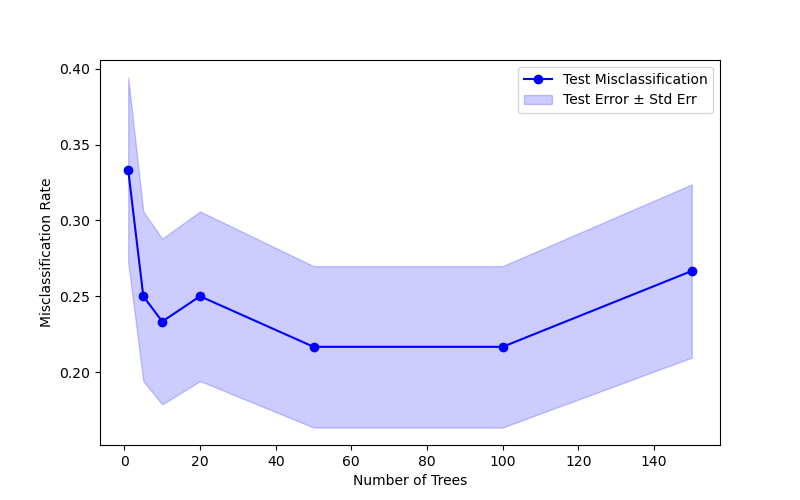
\includegraphics[width=0.5\textwidth]{fig/misclassification_vs_trees}
    \caption{Misclassification Rate vs. Number of Trees in Random Forest}
    \label{fig:misclassification_plot}
\end{figure}
%Key observations include:
%\begin{itemize}
%\item The misclassification rate decreases initially, reaching its lowest point at around \textbf{50 trees}.
%\item Beyond 50 trees, the rate stabilizes, showing no notable improvement.
%\item The standard error remains steady, suggesting consistent performance once the forest is sufficiently large.
%\end{itemize}
Key observations include: the misclassification rate decreases initially, reaching its lowest point at around \textbf{50 trees}. Beyond 50 trees, the rate stabilizes, showing no notable improvement. The standard error remains steady, suggesting consistent performance once the forest is sufficiently large.
%These results match random forest theory: adding more trees reduces variance and improves performance, but after a certain point, the benefits slow down. For this dataset, 50 trees are enough, as adding more trees does not significantly improve the results.

%------------------------------------------------

\section*{Part 2: Variable Importance Analysis}

\subsection*{Methodology}

\subsubsection*{Permutation-Based Feature Importance}


We measured variable importance in random forests using out-of-bag (OOB) samples. For each tree, OOB samples (data not used in training) are passed through the tree to record prediction accuracy. To assess a variable's importance, its values in the OOB samples are permuted, and the accuracy is recalculated. The decrease in accuracy across all trees, caused by this permutation, serves as the variable's importance measure. This approach simulates removing the variable's contribution, offering a reliable estimate of its predictive strength\cite{ESL}.

\subsection*{Results}


\subsubsection*{Variable Importance and Root Frequency}

To analyze the importance of features in the dataset, we computed the variable importance for a random forest with \( n = 100 \) trees. For comparison, we also calculated the frequency of features appearing as the root split in 100 non-random trees trained on randomized data.

\begin{figure}[h!]
    \centering
    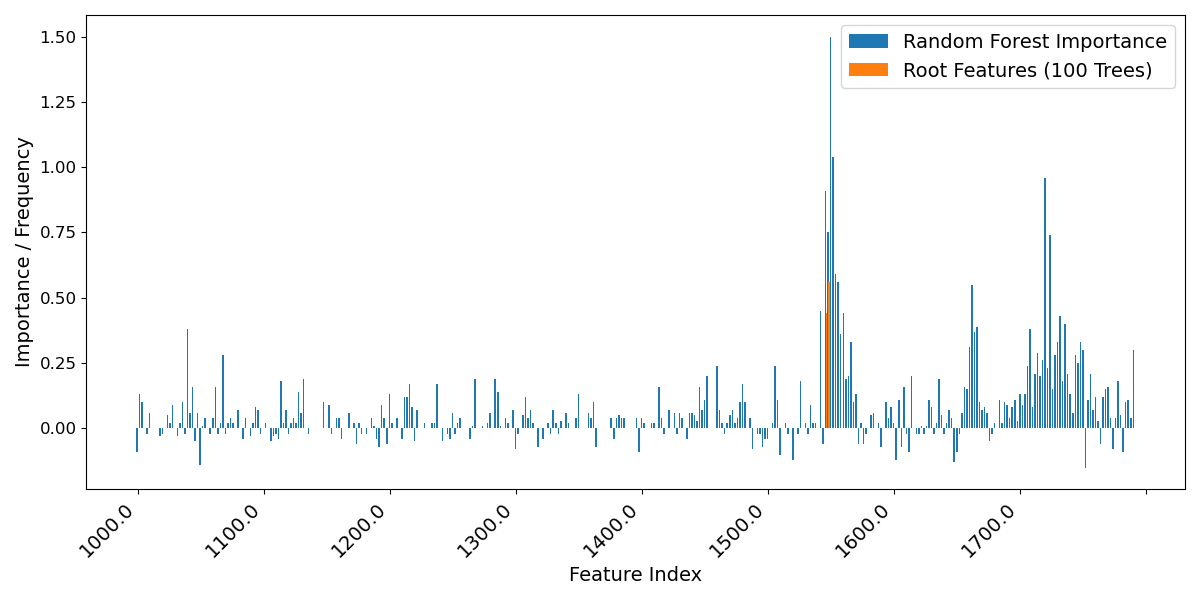
\includegraphics[width=0.5\textwidth]{fig/variable_importance}
    \caption{Variable Importance (Random Forest) vs. Root Frequency (Non-Random Trees)}
    \label{fig:variable_importance}
\end{figure}

Figure~\ref{fig:variable_importance} reveals that only two features appeared as the root split in non-random trees:
\begin{itemize}
\item
 \textbf{Feature 1548.0}: Ranked 5th in importance by the random forest, it appeared as the root split in 56\% of non-random trees.
\item
\textbf{Feature 1546.0}: Ranked 4th in importance by the random forest, it appeared as the root split in 44\% of non-random trees.
\end{itemize}



%------------------------------------------------

\section*{Part 3: Extended Variable Importance}


\subsubsection*{Extended Variable Importance to Combinations of Three Variables}
To extend variable importance to combinations of three variables, we implemented the \textbf{importance3()} method. This approach permutes three features simultaneously and measures the drop in prediction accuracy, capturing critical feature interactions. We applied this method to a random forest with n=1000 trees and compared it to the single-feature importance method by comparing the performance of a tree on the best three features identified by each method.

\subsubsection*{Tree Structure-Based Importance}
In scenarios where the original data is unavailable but a pre-built forest exists, we implemented the \textbf{importance3\_structure()} method. This method identifies the best combination of three variables by analyzing the structure of the trees in the forest:
\begin{itemize}
    \item For each tree, we extract the features used in its splits and count how often each combination of three features appears together.
    \item The combination with the highest frequency across all trees is selected as the most important.
\end{itemize}

\subsubsection*{Comparison of Classification Trees}

\begin{table}[h!]
\centering
\caption{Classification Tree Performance Using Top 3 Features Identified by Different Methods}
\label{tab:feature_performance}
\begin{tabular}{|l|c|c|}
\hline
\textbf{Importance Method} & \textbf{Top 3 Features} & \textbf{Accuracy} \\ \hline
Single-Feature & ['1548', '1552', '1550'] & 58.33\% \\ \hline
3-Feature Combination & ['1660', '1550', '1558'] & 63.33\% \\ \hline
Tree Structure-Based & ['1784', '1546', '1554'] & 63.33\% \\ \hline
\end{tabular}
\end{table}

%\subsubsection*{Key Observations}
%\begin{itemize}
%    \item The classification trees built using the top 3-feature combinations (\textbf{importance3} and \textbf{importance3\_structure}) outperformed the tree built using the top 3 single features, achieving an accuracy of \textbf{63.33\%} compared to \textbf{58.33\%}.
%    \item Both 3-feature combination methods (\textbf{importance3} and \textbf{importance3\_structure}) performed equally well, suggesting that considering feature interactions is crucial for improving model performance.
%    \item The \textbf{importance3\_structure} method, which relies on the structure of the pre-built forest, identified a different combination of features (\textbf{['1784.0', '1546.0', '1554.0']}) but achieved the same accuracy as \textbf{importance3}. This demonstrates that the tree structure-based approach is effective even without access to the original data.
%\end{itemize}

%\subsubsection*{Why the Tree Structure-Based Method Works Well}
%
%Since we only have access to the random forest and not the original data, the method analyzes all splits in the trees to extract the features used. By tracking the frequency of 3-feature combinations across the forest, it selects the combination that appears most frequently. This works well because features that are frequently used together in splits are likely to capture important patterns in the data and effectively partition it. In a random forest, features that are frequently used in splits are those that provide the most information gain or Gini impurity reduction. If a combination of features is frequently used together, it suggests that these features collectively contribute to better splits, meaning they capture important patterns in the data.
%
%
%\subsubsection*{Why Counting Frequencies at All Levels is Important}
%
%Counting frequencies of all features at every level, rather than just high-level features, ensures a comprehensive understanding of the data. High-level splits capture global patterns, while lower-level splits refine these with localized, nuanced interactions. Ignoring lower levels risks missing critical feature combinations that only become apparent deeper in the trees. Additionally, random forests introduce variability across trees, so evaluating all levels ensures robustness and avoids bias. This approach balances global and local importance, capturing hierarchical interactions and leading to more accurate feature selection and data partitioning.

\subsubsection*{Why the Tree Structure-Based Method Works Well}

The tree structure-based method works effectively because it analyzes all splits in the random forest to extract feature usage, even without access to the original data. By tracking the frequency of 3-feature combinations across the forest, it identifies the most frequently used combinations, which are likely to capture important patterns and partition the data effectively. Features frequently used in splits are those that provide the most information gain or Gini impurity reduction, indicating their importance. Counting frequencies at all levels, not just high-level splits, ensures a comprehensive understanding of the data. High-level splits capture global patterns, while lower-level splits refine these with more detailed, localized interactions. Ignoring lower levels risks missing critical feature combinations that only become apparent deeper in the trees. Additionally, evaluating all levels ensures robustness to variability across trees, avoids bias, and balances global and local importance, leading to more accurate feature selection and data partitioning.






%------------------------------------------------

%\section*{Discussion}


%------------------------------------------------


%----------------------------------------------------------------------------------------
%	REFERENCE LIST
%----------------------------------------------------------------------------------------
\bibliographystyle{unsrt}
\bibliography{report}


\end{document}